% Drawing 154/01-17 -- folder 154, batch 01, archive page 15 (PDF page 16).
% Transcription: figure en tête : un arrangement de pseudo-droites orange et une droite jaune $D$ ; un arc en pointillé vert, partant de $D$, longe une des droites orange jusqu'à un sommet, où il tourne
% Kind: arrangement with a line D and a dashed arc. Method 2 (schematic redraw from the facsimile). Status: ok.
% Notes: Four orange lines and the thick yellow-green line D; the dashed green arc leaves D where the long orange line cuts it, runs just above that line up to its crossing with the third line (a marked vertex), turns there and comes back down to D in dots. Vertices computed; the figure runs to the edge of the scan on the right. No letter is written in the figure. Redrawn 2026-11-12 (issue 128): to check again.
% Coordinates: 1 unit = 1 mm = 1/100 of the crop width (bbox in page fractions: [0.1, 0.07, 0.31, 0.165]).
% Redrawn by Claude (claude-fable-5-2), issue #128, 2026-11-12; not checked by a human; not compiled (no TeX in the session).
% Rights: reproduces part of the work -- behind RENDER_TRANSCRIPTS, never published by itself.
\documentclass[tikz,border=3pt]{standalone}
\usepackage{amsmath,amssymb}
\usetikzlibrary{patterns,arrows.meta}
\tikzset{Or/.style={orange!90!black}, Ye/.style={yellow!80!orange}, Lg/.style={green!60!black!70}, pencil/.style={black!45}, struck/.style={black!35}, mpt/.style={circle,draw,inner sep=1.3pt}, pt/.style={circle,fill,inner sep=0.9pt}, opt/.style={circle,draw,fill=white,inner sep=1.1pt}}
\begin{document}
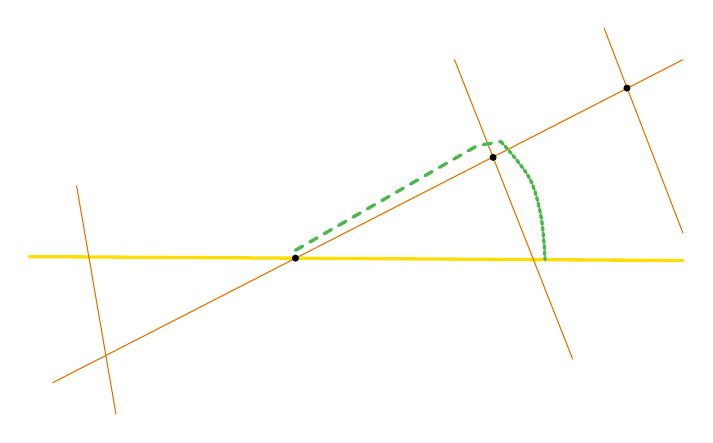
\begin{tikzpicture}[x=1mm,y=1mm,line cap=round,line join=round,font=\scriptsize]
\draw[Ye,very thick] (17,-41) -- (100,-41.5);
\draw[Or] (23,-32) -- (28,-61);
\draw[Or] (20,-57) -- (100,-16);
\draw[Or] (71,-16) -- (86,-54);
\draw[Or] (90,-12) -- (100,-38);
\draw[Lg,dashed,very thick] (50.8,-40.2) -- (73.9,-26.9) -- (76.9,-26.4);
\draw[Lg,densely dotted,very thick] plot[smooth, tension=0.55] coordinates {(76.9,-26.4) (80.5,-31) (82,-36) (82.5,-41.4)};
\node[pt] at (75.9,-28.4) {};
\node[pt] at (92.9,-19.6) {};
\node[pt] at (50.8,-41.2) {};
\end{tikzpicture}
\end{document}
